\documentclass[tikz,border=4pt]{standalone}
\usepackage{amsmath}
\begin{document}
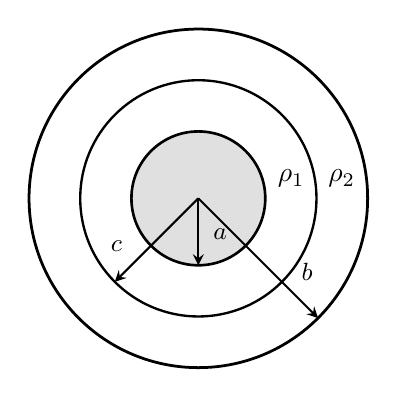
\begin{tikzpicture}[>=stealth, thick, scale=1.0]
  % Inner spherical electrode of radius a = 0.85 (subtle gray fill for legibility in light & dark modes)
  \draw[line width=0.95pt, fill=black!12] (0, 0) circle (0.85);
  % Interface of radius c = 1.50
  \draw[line width=0.85pt] (0, 0) circle (1.50);
  % Outer spherical shell electrode of radius b = 2.15
  \draw[line width=1.0pt] (0, 0) circle (2.15);

  % Radius arrows a, c, b
  \draw[->, line width=0.75pt] (0, 0) -- (0, -0.85);
  \node[right, font=\small] at (0.06, -0.45) {$a$};

  \draw[->, line width=0.75pt] (0, 0) -- (-1.06, -1.06);
  \node[above left, font=\small] at (-0.84, -0.80) {$c$};

  \draw[->, line width=0.75pt] (0, 0) -- (1.52, -1.52);
  \node[above right, font=\small] at (1.18, -1.18) {$b$};

  % Resistivity labels rho_1 (a < r < c) and rho_2 (c < r < b)
  \node at (1.18, 0.25) {$\rho_1$};
  \node at (1.82, 0.25) {$\rho_2$};
\end{tikzpicture}
\end{document}
